\documentclass{article}
% translate with >> pdflatex -shell-escape <file>

% This file is an extract of the PGFPLOTS manual, copyright by Christian Feuersaenger.
% 
% Feel free to use it as long as you cite the pgfplots manual properly.
%
% See
%   http://pgfplots.sourceforge.net/pgfplots.pdf
% for the complete manual.
%
% Any required input files (for <plot table> or <plot file> or the table package) can be downloaded
% at
% http://www.ctan.org/tex-archive/graphics/pgf/contrib/pgfplots/doc/latex/
% and
% http://www.ctan.org/tex-archive/graphics/pgf/contrib/pgfplots/doc/latex/plotdata/

\usepackage{pgfplots}
\pgfplotsset{compat=newest}

\pagestyle{empty}
\usetikzlibrary{patterns}

\begin{document}
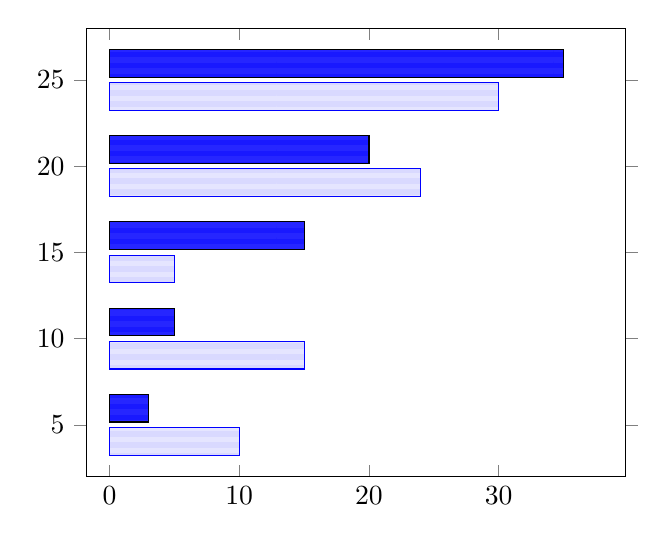
\begin{tikzpicture}
\begin{axis}[xbar,enlargelimits=0.15]
\addplot
[draw=blue,pattern=horizontal lines light blue] 
coordinates
	{(10,5) (15,10) (5,15) (24,20) (30,25)};

\addplot
[draw=black,pattern=horizontal lines dark blue] 
coordinates 
	{(3,5) (5,10) (15,15) (20,20) (35,25)};
\end{axis}
\end{tikzpicture}
\end{document}
